\documentclass{article}
\usepackage{parskip}
\usepackage{amsmath}
% use UTF8 encoding
\usepackage[utf8]{inputenc}
% use KoTeX package for Korean
\usepackage{kotex}
\usepackage{hyperref}
\usepackage{enumitem}
\usepackage{matlab-prettifier}
\usepackage{geometry}
\usepackage{graphicx}
\usepackage{hyperref}
\usepackage{subcaption,lipsum}

\hypersetup{
    colorlinks=true,
    linkcolor=blue,
    filecolor=magenta,      
    urlcolor=cyan,
    pdftitle={Overleaf Example},
    pdfpagemode=FullScreen,
}

\geometry{
    a4paper,
    left=30mm,
    right=30mm,
    top=30mm,
    bottom=40mm
 }

\hypersetup{
    colorlinks=true,   
    urlcolor=red,
}

\begin{document}

\title{Assignment 5}
\author{20180282 Jimin Park}
\maketitle


\begin{enumerate}
    \item We can rewrite the first equation as below: \begin{align}
        \label{eqn:diff_eq}
        y^\prime - \frac{1}{t}y = 1.
    \end{align} Now let's find the integrating factor $I(t)$: \begin{align*}
        \begin{split}
            I(t) &= \exp \left(\int -\frac{1}{t}\right)
            \\ &= \exp \left(\ln\left(\frac{1}{t}\right)+C\right)
            \\ &= \exp(C) \frac{1}{t}.
        \end{split}
    \end{align*} Here, I'll take $C=0$ for simplicity of calculation. Then we get \begin{align}
        \label{eqn:integrating_factor}
        I(t) = \frac{1}{t}
    \end{align} Now, multiply the integrating factor (\ref{eqn:integrating_factor}) to the both side of the differential equation (\ref{eqn:diff_eq}). Then we can rewrite the equation by \begin{align}
        \label{eqn:transformed_diff_eq}
        \frac{d}{dt}\left(\frac{1}{t}y\right) = \frac{1}{t}.
    \end{align} By integrating \ref{eqn:transformed_diff_eq} w.r.t. $t$, we get \begin{align}
        \label{eqn:eq_with_constant}
        \frac{1}{t}y = \ln(t) + K
    \end{align} Here, we can use the initial condition $y(1)=2$. By plugging in $t=1, y=2$ to \ref{eqn:eq_with_constant}, we get $K=2$. Hence, we solved the differnetial equation and can write $y$ only by $t$: \begin{align}
        \label{eqn:diff_eq_ans}
        y=t\ln(t)+2t
    \end{align}
    \item Below is the code for modified Euler method to solve the given differential equation: \begin{lstlisting}[frame=single, numbers=left, style=Matlab-editor]
syms t w;
f(t,w) = 1 + w/t;
y(t) = t*log(t) + 2*t;

for h=[1/10, 1/20, 1/40]
    [~, y_values] = Exact_Values(h, y);
    [t_values, w_values] = Modified_Euler_Method(h, f);
    [error_values, max_error] = Error(y_values, w_values);
    fprintf('----------------------------------------------------\n');
    fprintf('Modified Euler method with h=1/%d:\n', 1/h);
    fprintf('Approximated values are:\n');
    disp(w_values);
    fprintf('Absolute errors for each values are\n');
    disp(error_values);
    fprintf('Maximum absolute error is: %e\n', max_error)
end

% last t_values and error_values are saved
% they are values associated with h=1/40
plot(t_values, error_values)
xlabel('x');
ylabel('error');

function [t_values, w_values] = Modified_Euler_Method(h, f)
    % for speed, i did preallocation
    numbs = 1/h + 1;
    t_values = 1:h:2;
    w_values = zeros(1, numbs);

    t = 1;
    w = 2;
    w_values(1) = w;
    for i=2:numbs
        w = w + h/2 * (f(t,w) + f(t+h,w+h*f(t,w)));
        w_values(i) = w;
        t = t + h;
    end
end

function [t_values, y_values] = Exact_Values(h, y)
    % for speed, i did preallocation
    numbs = 1/h + 1;
    t_values = 1:h:2;
    y_values = zeros(1, numbs);

    t = 1;
    for i=1:numbs
        y_values(i) = y(t);
        t = t + h;
    end
end

function [error_values, max_error] = Error(exact_values, approx_values)
    error_values = abs(exact_values - approx_values);
    max_error = max(error_values);
end
    \end{lstlisting} If we run this code in MATLAB, then we get the following result: \begin{lstlisting}[frame=single, numbers=left, style=Matlab-editor]
----------------------------------------------------
Modified Euler method with h=1/10:
Approximated values are:
    2.0000    2.3045    2.6182    2.9402    3.2700    3.6069    3.9505    4.3003    4.6561    5.0174    5.3839
Absolute errors for each values are
         0    0.0003    0.0006    0.0008    0.0011    0.0013    0.0015    0.0017    0.0020    0.0022    0.0024
Maximum absolute error is: 2.356042e-03
----------------------------------------------------
Modified Euler method with h=1/20:
Approximated values are:
    2.0000    2.1512    2.3048    2.4606    2.6186    2.7787    2.9409    3.1049    3.2708    3.4385    3.6079    3.7789    3.9516    4.1259    4.3016    4.4789    4.6575    4.8376    5.0190    5.2017    5.3857
Absolute errors for each values are
   1.0e-03 *

         0    0.0392    0.0767    0.1128    0.1475    0.1812    0.2138    0.2456    0.2765    0.3067    0.3363    0.3653    0.3937    0.4217    0.4492    0.4763    0.5031    0.5295    0.5556    0.5814    0.6069
Maximum absolute error is: 6.068784e-04
----------------------------------------------------
Modified Euler method with h=1/40:
Approximated values are:
    2.0000    2.0753    2.1512    2.2277    2.3048    2.3825    2.4607    2.5395    2.6187    2.6986    2.7789    2.8597    2.9410    3.0228    3.1051    3.1878    3.2710    3.3546    3.4387    3.5232    3.6081    3.6935    3.7792    3.8654    3.9519    4.0388    4.1262    4.2139    4.3020    4.3904    4.4792    4.5684    4.6579    4.7478    4.8380    4.9285    5.0194    5.1106    5.2021    5.2940    5.3861
Absolute errors for each values are
   1.0e-03 *

         0    0.0050    0.0100    0.0148    0.0195    0.0242    0.0287    0.0332    0.0375    0.0418    0.0461    0.0503    0.0544    0.0584    0.0624    0.0664    0.0703    0.0741    0.0779    0.0817    0.0854    0.0891    0.0928    0.0964    0.1000    0.1036    0.1071    0.1106    0.1141    0.1175    0.1209    0.1243    0.1277    0.1310    0.1344    0.1377    0.1410    0.1443    0.1475    0.1508    0.1540
Maximum absolute error is: 1.539778e-04
    \end{lstlisting} And we also get the error graph Fig.\ref{fig:Modified_Euler_Method_Error_Graph} for $h=1/40$ case. \begin{figure}[h] %%% t: top, b: bottom, h: here
        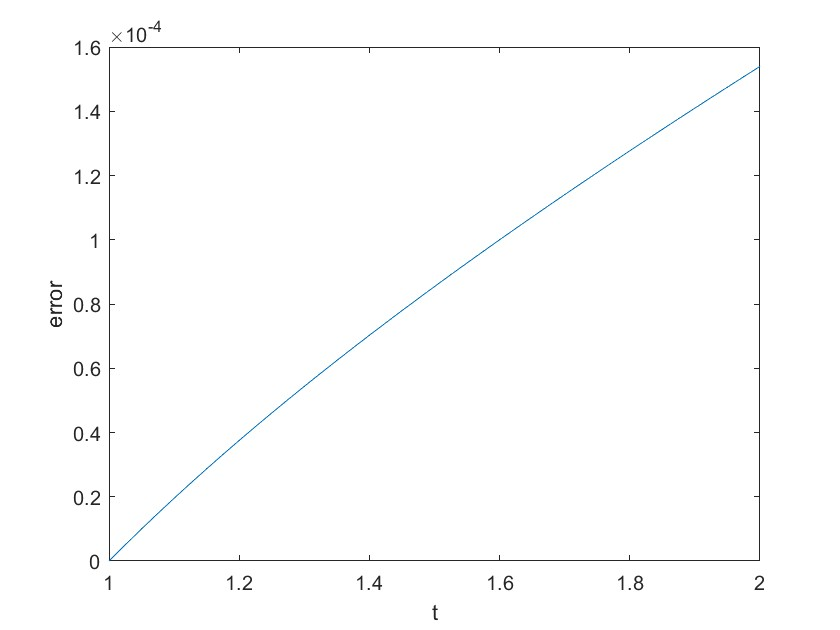
\includegraphics[width=0.9\textwidth]{assignment_5_2_fig.jpg}
        \centering
        \caption{Plotting of error of Modified Euler method}
        \label{fig:Modified_Euler_Method_Error_Graph}
    \end{figure}
    
    Now, let's discuss the reduction of errors. We learned that the Modified Euler method have LTE $O(h^2)$. And we also learned that order of LTE gurantee the order of the global error when function used for updating $w$ values satisfies a Lipschitz condition in the variable $w$. Hence, we can say that the global error for the Modified Euler method is $O(h^2)$. In the code, we use $h=1/10, 1/20, 1/40$ in this order, and the magnitude of h is multipled by $1/2$ in this order. It means the global error will be reduced by about 4 times. Remind that the maximum absolute errors are $2.356042\times 10^{-3}$, $6.068784\times 10^{-4}$, and $1.539778\times 10^{-4}$ when $h=1/10, 1/20,$ and $1/40$, respectively. And the rate of these errors are: \begin{align*}
        \frac{2.356042\times 10^{-3}}{6.068784\times 10^{-4}} \approx 3.8822,
        \\ \frac{6.068784\times 10^{-4}}{1.539778\times 10^{-4}} \approx 3.9413.
    \end{align*} These rates are all near 4, and this fact well support the theorem that error for the Modified Euler method is $O(h^2)$
    \item \begin{enumerate}[wide=10pt]
        \item Below is the code for RK4 method to solve the given differential equation: \begin{lstlisting}[frame=single, numbers=left, style=Matlab-editor]
syms t w;
f(t,w) = 1 + w/t;
y(t) = t*log(t) + 2*t;

for h=[1/10, 1/20, 1/40]
    [~, y_values] = Exact_Values(h, y);
    [t_values, w_values] = RK4(h, f);
    [error_values, max_error] = Error(y_values, w_values);
    fprintf('----------------------------------------------------\n');
    fprintf('RK4 method with h=1/%d:\n', 1/h);
    fprintf('Approximated values are:\n');
    disp(w_values)
    fprintf('Absolute errors for each values are\n');
    disp(error_values);
    fprintf('Maximum absolute error is: %e\n', max_error)
end

% last t_values and error_values are saved
% they are values associated with h=1/40
plot(t_values, error_values)
xlabel('x');
ylabel('error');

function [t_values, w_values] = RK4(h, f)
    % for speed, i did preallocation
    numbs = 1/h + 1;
    t_values = 1:h:2;
    w_values = zeros(1, numbs);

    t = 1;
    w = 2;
    w_values(1) = w;
    for i=2:numbs
        K1 = h * f(t,w);
        K2 = h * f(t+h/2, w+K1/2);
        K3 = h * f(t+h/2, w+K2/2);
        K4 = h * f(t+h, w+K3);
        w = w + (K1+2*K2+2*K3+K4)/6;
        t = t + h;

        w_values(i) = w;
    end
end

function [t_values, y_values] = Exact_Values(h, y)
    % for speed, i did preallocation
    numbs = 1/h + 1;
    t_values = 1:h:2;
    y_values = zeros(1, numbs);

    t = 1;
    for i=1:numbs
        y_values(i) = y(t);
        t = t + h;
    end
end

function [error_values, max_error] = Error(exact_values, approx_values)
    error_values = abs(exact_values - approx_values);
    max_error = max(error_values);
end
        \end{lstlisting} If we run this code in MATLAB, then we get the following result: \begin{lstlisting}[frame=single, numbers=left, style=Matlab-editor]
----------------------------------------------------
RK4 method with h=1/10:
Approximated values are:
    2.0000    2.3048    2.6188    2.9411    3.2711    3.6082    3.9520    4.3021    4.6580    5.0195    5.3863
Absolute errors for each values are
   1.0e-05 *

         0    0.0272    0.0485    0.0661    0.0811    0.0944    0.1064    0.1175    0.1280    0.1379    0.1475
Maximum absolute error is: 1.474767e-06
----------------------------------------------------
RK4 method with h=1/20:
Approximated values are:
    2.0000    2.1512    2.3048    2.4607    2.6188    2.7789    2.9411    3.1051    3.2711    3.4388    3.6082    3.7793    3.9520    4.1263    4.3021    4.4793    4.6580    4.8381    5.0195    5.2023    5.3863
Absolute errors for each values are
   1.0e-07 *

         0    0.0938    0.1759    0.2486    0.3138    0.3729    0.4270    0.4771    0.5238    0.5677    0.6092    0.6487    0.6864    0.7228    0.7579    0.7919    0.8250    0.8572    0.8888    0.9198    0.9502
Maximum absolute error is: 9.501746e-08
----------------------------------------------------
RK4 method with h=1/40:
Approximated values are:
    2.0000    2.0753    2.1512    2.2277    2.3048    2.3825    2.4607    2.5395    2.6188    2.6986    2.7789    2.8598    2.9411    3.0229    3.1051    3.1879    3.2711    3.3547    3.4388    3.5233    3.6082    3.6935    3.7793    3.8655    3.9520    4.0390    4.1263    4.2140    4.3021    4.3905    4.4793    4.5685    4.6580    4.7479    4.8381    4.9286    5.0195    5.1107    5.2023    5.2941    5.3863
Absolute errors for each values are
   1.0e-08 *

         0    0.0309    0.0596    0.0865    0.1118    0.1355    0.1579    0.1791    0.1992    0.2184    0.2367    0.2542    0.2710    0.2872    0.3028    0.3178    0.3323    0.3464    0.3601    0.3734    0.3864    0.3990    0.4114    0.4235    0.4353    0.4469    0.4583    0.4695    0.4805    0.4914    0.5021    0.5126    0.5230    0.5333    0.5435    0.5535    0.5634    0.5733    0.5830    0.5927    0.6023
Maximum absolute error is: 6.022818e-09
        \end{lstlisting} And we also get the error graph Fig.\ref{fig:RK2_Method_Error_Graph} for $h=1/40$ case. \begin{figure}[h] %%% t: top, b: bottom, h: here
            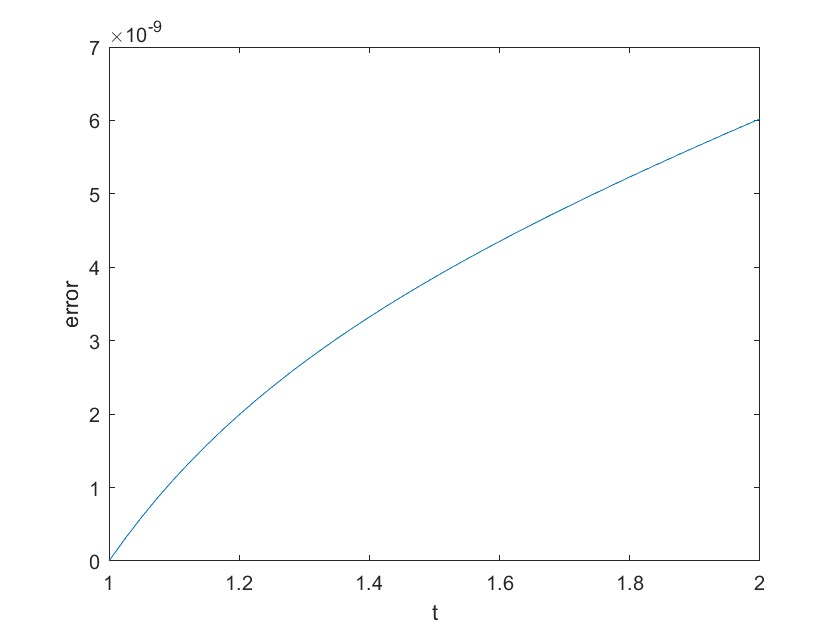
\includegraphics[width=0.9\textwidth]{assignment_5_3_1_fig.jpg}
            \centering
            \caption{Plotting of error of RK2 method}
            \label{fig:RK2_Method_Error_Graph}
        \end{figure}

        Now, let's discuss the reduction of errors. We learned that the RK4 method have LTE $O(h^4)$. Using the similar process for solution of problem 2, the global error will be reduced by about 16 times as $h$ is reduced by 2 times. Remind that the maximum absolute errors are $1.474767\times 10^{-6}$, $9.501746\times 10^{-8}$, and $6.022818\times 10^{-9}$ when $h=1/10, 1/20,$ and $1/40$, respectively. And the rate of these errors are: \begin{align*}
            \frac{1.474767\times 10^{-6}}{9.501746\times 10^{-8}} \approx 15.521,
            \\ \frac{9.501746\times 10^{-8}}{6.022818\times 10^{-9}} \approx 15.776.
        \end{align*} These rates are all near 16, and this fact well support the theorem that error for the RK4 method is $O(h^4)$.
        \item Below is the code for Adams 4th-Order Predictor-Corrector method to solve the given differential equation: \begin{lstlisting}[frame=single, numbers=left, style=Matlab-editor]
syms t w;
f(t,w) = 1 + w/t;
y(t) = t*log(t) + 2*t;

for h=[1/10, 1/20, 1/40]
    [~, y_values] = Exact_Values(h, y);
    [t_values, w_values] = Adams_4th_Order_Predictor_Corrector(h, f);
    [error_values, max_error] = Error(y_values, w_values);
    fprintf('----------------------------------------------------\n');
    fprintf('Adams 4th-order predictor-corrector method with h=1/%d:\n', 1/h);
    fprintf('Approximated values are:\n');
    disp(w_values)
    fprintf('Absolute errors for each values are\n');
    disp(error_values);
    fprintf('Maximum absolute error is: %e\n', max_error)
end

% last t_values and error_values are saved
% they are values associated with h=1/40
plot(t_values, error_values)
xlabel('x');
ylabel('error');

function [t_values, w_values] = Adams_4th_Order_Predictor_Corrector(h, f)
    % for speed, i did preallocation
    numbs = 1/h + 1;
    t_values = 1:h:2;
    w_values = zeros(1, numbs);

    t = 1;
    w = 2;
    w_values(1) = w;

    % RK4 for starting values
    for i=2:4
        K1 = h * f(t,w);
        K2 = h * f(t+h/2, w+K1/2);
        K3 = h * f(t+h/2, w+K2/2);
        K4 = h * f(t+h, w+K3);
        w = w + (K1+2*K2+2*K3+K4)/6;
        t = t + h;

        w_values(i) = w;
    end

    % Set starting pts
    w0 = w_values(1);
    w1 = w_values(2);
    w2 = w_values(3);
    w3 = w_values(4);
    t0 = t_values(1);
    t1 = t_values(2);
    t2 = t_values(3);
    t3 = t_values(4);

    % Do predictor corrector method
    for i=5:numbs
        t = t + h;
        % predict w_i
        w = w3 + h*(55*f(t3,w3)-59*f(t2,w2)+37*f(t1,w1)-9*f(t0,w0))/24;
        % correct w_i
        w = w3 + h*(9*f(t,w)+19*f(t3,w3)-5*f(t2,w2)+f(t1,w1))/24;

        w_values(i) = w;

        % reset w's and t's
        t0 = t1;
        t1 = t2;
        t2 = t3;
        t3 = t;
        w0 = w1;
        w1 = w2;
        w2 = w3;
        w3 = w;
    end
end

function [t_values, y_values] = Exact_Values(h, y)
    % for speed, i did preallocation
    numbs = 1/h + 1;
    t_values = 1:h:2;
    y_values = zeros(1, numbs);

    t = 1;
    for i=1:numbs
        y_values(i) = y(t);
        t = t + h;
    end
end

function [error_values, max_error] = Error(exact_values, approx_values)
    error_values = abs(exact_values - approx_values);
    max_error = max(error_values);
end
        \end{lstlisting} If we run this code in MATLAB, then we get the following result: \begin{lstlisting}[frame=single, numbers=left, style=Matlab-editor]
----------------------------------------------------
Adams 4th-order predictor-corrector method with h=1/10:
Approximated values are:
    2.0000    2.3048    2.6188    2.9411    3.2711    3.6082    3.9520    4.3021    4.6580    5.0195    5.3863
Absolute errors for each values are
   1.0e-05 *

         0    0.0272    0.0485    0.0661    0.1046    0.1388    0.1693    0.1968    0.2222    0.2457    0.2679
Maximum absolute error is: 2.679057e-06
----------------------------------------------------
Adams 4th-order predictor-corrector method with h=1/20:
Approximated values are:
    2.0000    2.1512    2.3048    2.4607    2.6188    2.7789    2.9411    3.1051    3.2711    3.4388    3.6082    3.7793    3.9520    4.1263    4.3021    4.4793    4.6580    4.8381    5.0195    5.2023    5.3863
Absolute errors for each values are
   1.0e-06 *

         0    0.0094    0.0176    0.0249    0.0488    0.0704    0.0900    0.1079    0.1245    0.1399    0.1543    0.1678    0.1807    0.1929    0.2046    0.2158    0.2266    0.2371    0.2473    0.2572    0.2668
Maximum absolute error is: 2.668425e-07
----------------------------------------------------
Adams 4th-order predictor-corrector method with h=1/40:
Approximated values are:
    2.0000    2.0753    2.1512    2.2277    2.3048    2.3825    2.4607    2.5395    2.6188    2.6986    2.7789    2.8598    2.9411    3.0229    3.1051    3.1879    3.2711    3.3547    3.4388    3.5233    3.6082    3.6935    3.7793    3.8655    3.9520    4.0390    4.1263    4.2140    4.3021    4.3905    4.4793    4.5685    4.6580    4.7479    4.8381    4.9286    5.0195    5.1107    5.2023    5.2941    5.3863
Absolute errors for each values are
   1.0e-07 *

         0    0.0031    0.0060    0.0087    0.0193    0.0294    0.0388    0.0477    0.0562    0.0642    0.0718    0.0791    0.0860    0.0927    0.0991    0.1052    0.1112    0.1169    0.1224    0.1278    0.1330    0.1381    0.1430    0.1479    0.1526    0.1572    0.1617    0.1661    0.1704    0.1747    0.1788    0.1830    0.1870    0.1910    0.1949    0.1988    0.2027    0.2064    0.2102    0.2139    0.2176
Maximum absolute error is: 2.175862e-08
        \end{lstlisting} And we also get the error graph Fig.\ref{fig:Adams_4th_Order_Predictor_Corrector_Method_Error_Graph} for $h=1/40$ case. \begin{figure}[h] %%% t: top, b: bottom, h: here
            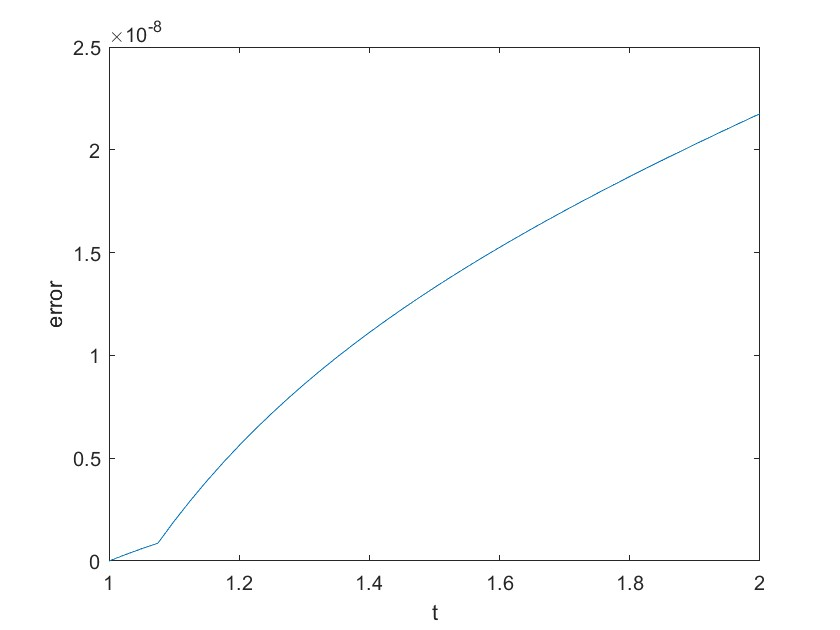
\includegraphics[width=0.9\textwidth]{assignment_5_3_2_fig.jpg}
            \centering
            \caption{Plotting of error of Adams 4th-Order Predictor-Corrector method}
            \label{fig:Adams_4th_Order_Predictor_Corrector_Method_Error_Graph}
        \end{figure}

        Now, let's discuss the reduction of errors. We learned that the Adams 4th-Order Predictor-Corrector method have LTE $O(h^4)$. Using the similar process for solution of problem 2, the global error will be reduced by about 16 times as $h$ is reduced by 2 times. Remind that the maximum absolute errors are $2.679057\times 10^{-6}$, $2.668425\times 10^{-7}$, and $2.175862\times 10^{-8}$ when $h=1/10, 1/20,$ and $1/40$, respectively. And the rate of these errors are: \begin{align*}
            \frac{2.679057\times 10^{-6}}{2.668425\times 10^{-7}} \approx 10.040,
            \\ \frac{2.668425\times 10^{-7}}{2.175862\times 10^{-8}} \approx 12.263.
        \end{align*} These rates are no that near 16. It can be happen since we just compare 3 $h$ values and $h$ is not that small. If we reduce $h$ more, the rate will approach to 16. To clarify it, I found more maximum absolute errors, for $h=1/80, 1/160,$ and $1/320$, and they are $1.565647\times 10^{-9}$, $1.052012\times 10^{-10}$, and $6.821210\times 10^{-12}$, respectively. Then the rate of erros are: \begin{align*}
            \frac{2.175862\times 10^{-8}}{1.565647\times 10^{-9}} \approx 13.898,
            \\ \frac{1.565647\times 10^{-9}}{1.052012\times 10^{-10}} \approx 14.882,
            \\ \frac{1.052012\times 10^{-10}}{6.821210\times 10^{-12}} \approx 15.423.
        \end{align*} These rates are all near 16, and this fact well support the theorem that error for the Adams 4th-Order Predictor-Corrector method is $O(h^4)$.
        \item Let’s compare these two methods in terms of three perspectives. \begin{enumerate}[wide=30pt]
            \item Accuracy perspective
            
            With the results of (a) and (b), in this differential equation problem, RK4 method is more accurate than the Adams 4th-Order Predictor-Corrector method. It may because Adams 4th-Order Predictor-Corrector method uses interpolation technique to predict the value, and in this problem, such technique may accumlate erros more  than RK4. But we can see both methods works well with error $O(h^4)$.
            \item Cost perspective
            
            Since the function value calculation requires a lot of calculation, it is expensive operation. And If we see the codes above, for each iteration, it seems that Adams 4th-Order Predictor-Corrector method do that operation 8 times while RK4 only do it 4 times. But actually, the essence of Adams method is predicting value using previous values, and we can reuse the previously calculated function values, which means that we only need to calculate function value once at each iteration. Hence if we design the code well, Adams 4th-Order Predictor-Corrector method is cost-effective than the RK4 method. Below is the code inspired by such idea. \begin{lstlisting}[frame=single, numbers=left, style=Matlab-editor]
syms t w;
f(t,w) = 1 + w/t;
y(t) = t*log(t) + 2*t;

for h=[1/10, 1/20, 1/40]
    [~, y_values] = Exact_Values(h, y);
    [t_values, w_values] = Adams_4th_Order_Predictor_Corrector(h, f);
    [error_values, max_error] = Error(y_values, w_values);
    fprintf('----------------------------------------------------\n');
    fprintf('Adams 4th-order predictor-corrector method with h=1/%d:\n', 1/h);
    fprintf('Approximated values are:\n');
    disp(w_values)
    fprintf('Absolute errors for each values are\n');
    disp(error_values);
    fprintf('Maximum absolute error is: %e\n', max_error)
end

% last t_values and error_values are saved
% they are values associated with h=1/40
plot(t_values, error_values)
xlabel('x');
ylabel('error');

function [t_values, w_values] = Adams_4th_Order_Predictor_Corrector(h, f)
    % for speed, i did preallocation
    numbs = 1/h + 1;
    t_values = 1:h:2;
    w_values = zeros(1, numbs);

    t = 1;
    w = 2;
    w_values(1) = w;

    % RK4 for starting values
    for i=2:4
        K1 = h * f(t,w);
        K2 = h * f(t+h/2, w+K1/2);
        K3 = h * f(t+h/2, w+K2/2);
        K4 = h * f(t+h, w+K3);
        w = w + (K1+2*K2+2*K3+K4)/6;
        t = t + h;

        w_values(i) = w;
    end

    % Set starting pts
    f0 = f(t_values(1), w_values(1));
    f1 = f(t_values(2), w_values(2));
    f2 = f(t_values(3), w_values(3));
    f3 = f(t_values(4), w_values(4));
    w3 = w_values(4);

    % Do predictor corrector method
    for i=5:numbs
        t = t + h;
        % predict w_i
        w = w3 + h*(55*f3-59*f2+37*f1-9*f0)/24;
        % correct w_i
        fw = f(t, w);
        w = w3 + h*(9*fw+19*f3-5*f2+f1)/24;

        w_values(i) = w;

        % reset values for iteration
        f0 = f1;
        f1 = f2;
        f2 = f3;
        f3 = fw;
        w3 = w;
    end
end

function [t_values, y_values] = Exact_Values(h, y)
    % for speed, i did preallocation
    numbs = 1/h + 1;
    t_values = 1:h:2;
    y_values = zeros(1, numbs);

    t = 1;
    for i=1:numbs
        y_values(i) = y(t);
        t = t + h;
    end
end

function [error_values, max_error] = Error(exact_values, approx_values)
    error_values = abs(exact_values - approx_values);
    max_error = max(error_values);
end
            \end{lstlisting} I measured the required calculating time using MATLAB 'tic-tok' method, putting it to the start and the end point of the function. RK4 method takes 0.199864, 0.371800, and 0.749810 seconds when $h=1/10, 1/20,$ and $1/40$, respectively. Original Adams 4th-Order Predictor-Corrector method takes 0.393645, 0.575866, and 1.280589 seconds when $h=1/10, 1/20,$ and $1/40$, respectively. It takes longer time than RK4 method. But new well-designed Adams 4th-Order Predictor-Corrector method just takes 0.131285, 0.210110, and 0.357412 seconds when $h=1/10, 1/20,$ and $1/40$, respectively. This is significantly faster than the RK4 method.
        \end{enumerate}
    \end{enumerate}
    \item Below is the code for RK4 method using the step size of $h=0.001$ to solve the given system of ordinary differential equations: \begin{lstlisting}[frame=single, numbers=left, style=Matlab-editor]
syms t w1 w2;
f(t,w1,w2) = [w1*(4-0.0003*w1-0.0004*w2), w2*(2-0.0002*w1-0.0001*w2)];

h = 0.01;

[t_values, w1_values, w2_values] = RK4(h, f);
fprintf('----------------------------------------------------\n');
fprintf('RK4 method with h=%f:\n', h);
fprintf(['Since there are too many values, ' ...
    'just print values with interval length 1/10, i.e., ' ...
    'only print it once every 10 times\n']);
fprintf('Approximated w1 values are:\n');
disp(w1_values(1:10:end));
fprintf('Approximated w2 values are:\n');
disp(w2_values(1:10:end));
fprintf('----------------------------------------------------\n');
k = 30;
fprintf(['To see the convergence of w1 and w2 values clearly, ' ...
    'print last %d values\n'], k);
fprintf('Last %d approximated w1 values are:\n', k);
disp(w1_values(end-k+1:end));
fprintf('Last %d approximated w2 values are:\n', k);
disp(w2_values(end-k+1:end));

f1 = figure('Name','x-w1 graph');
plot(t_values, w1_values);
xlabel('x');
ylabel('w1');
f2 = figure('Name','x-w2 graph');
plot(t_values, w2_values);
xlabel('x');
ylabel('w2');

function [t_values, w1_values, w2_values] = RK4(h, f)
    % for speed, i did preallocation
    numbs = 4/h + 1;
    t_values = 0:h:4;
    w1_values = zeros(1, numbs);
    w2_values = zeros(1, numbs);

    t = 0;
    w1 = 10000;
    w2 = 10000;
    w1_values(1) = w1;
    w2_values(1) = w2;
    for i=2:numbs
        K1 = h * f(t,w1,w2);
        K2 = h * f(t+h/2, w1+K1(1)/2, w2+K1(2)/2);
        K3 = h * f(t+h/2, w1+K2(1)/2, w2+K2(2)/2);
        K4 = h * f(t+h, w1+K3(1), w2+K3(2));
        % put double for fast calculation
        w1 = w1 + double((K1(1)+2*K2(1)+2*K3(1)+K4(1))/6);
        w2 = w2 + double((K1(2)+2*K2(2)+2*K3(2)+K4(2))/6);
        t = t + h;

        w1_values(i) = w1;
        w2_values(i) = w2;
    end
end
    \end{lstlisting} If we run this code in MATLAB, then we get the following result: \begin{lstlisting}[frame=single, numbers=left, style=Matlab-editor]
----------------------------------------------------
RK4 method with h=0.010000:
Since there are too many values, just print values with interval length 1/10, i.e., only print it once every 10 times
Approximated w1 values are:
   1.0e+04 *

    1.0000    0.7804    0.6527    0.5675    0.5049    0.4553    0.4134    0.3764    0.3425    0.3106    0.2802    0.2509    0.2227    0.1956    0.1698    0.1454    0.1228    0.1021    0.0836    0.0673    0.0532    0.0414    0.0317    0.0239    0.0178    0.0130    0.0094    0.0068    0.0048    0.0034    0.0023    0.0016    0.0011    0.0008    0.0005    0.0004    0.0002    0.0002    0.0001    0.0001    0.0001
Approximated w2 values are:
   1.0e+04 *

    1.0000    0.9307    0.8999    0.8901    0.8936    0.9064    0.9263    0.9518    0.9823    1.0171    1.0557    1.0980    1.1435    1.1919    1.2427    1.2955    1.3497    1.4045    1.4593    1.5133    1.5657    1.6157    1.6629    1.7066    1.7466    1.7827    1.8148    1.8431    1.8677    1.8890    1.9072    1.9227    1.9358    1.9468    1.9560    1.9637    1.9701    1.9754    1.9797    1.9833    1.9863
----------------------------------------------------
To see the convergence of w1 and w2 values clearly, print last 30 values
Last 30 approximated w1 values are:
    1.5846    1.5239    1.4655    1.4093    1.3553    1.3033    1.2533    1.2052    1.1589    1.1143    1.0715    1.0303    0.9907    0.9525    0.9159    0.8806    0.8467    0.8140    0.7826    0.7525    0.7234    0.6955    0.6687    0.6428    0.6180    0.5941    0.5712    0.5491    0.5279    0.5074
Last 30 approximated w2 values are:
   1.0e+04 *

    1.9758    1.9763    1.9768    1.9772    1.9776    1.9781    1.9785    1.9789    1.9793    1.9797    1.9801    1.9805    1.9809    1.9813    1.9816    1.9820    1.9823    1.9827    1.9830    1.9833    1.9837    1.9840    1.9843    1.9846    1.9849    1.9852    1.9855    1.9858    1.9860    1.9863
    \end{lstlisting} And we also get the w1 and w2 graph Fig.\ref{fig:RK4_Method_w1_And_w2_Graph}. \begin{figure}[h] %%% t: top, b: bottom, h: here
        \begin{subfigure}{.5\textwidth}
            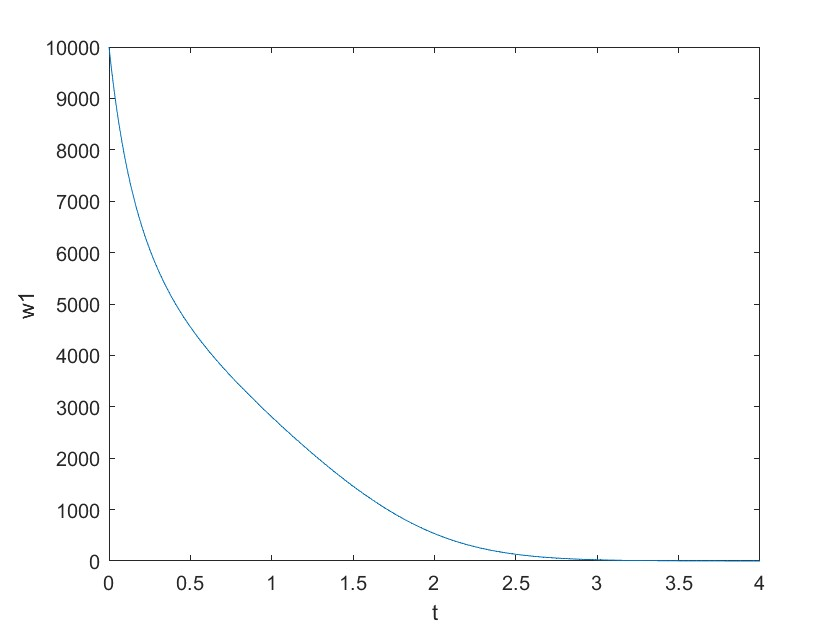
\includegraphics[width=\textwidth]{assignment_5_4_1_fig.jpg}
            \centering
            \caption{w1 graph}
        \end{subfigure}%
        \begin{subfigure}{.5\textwidth}
            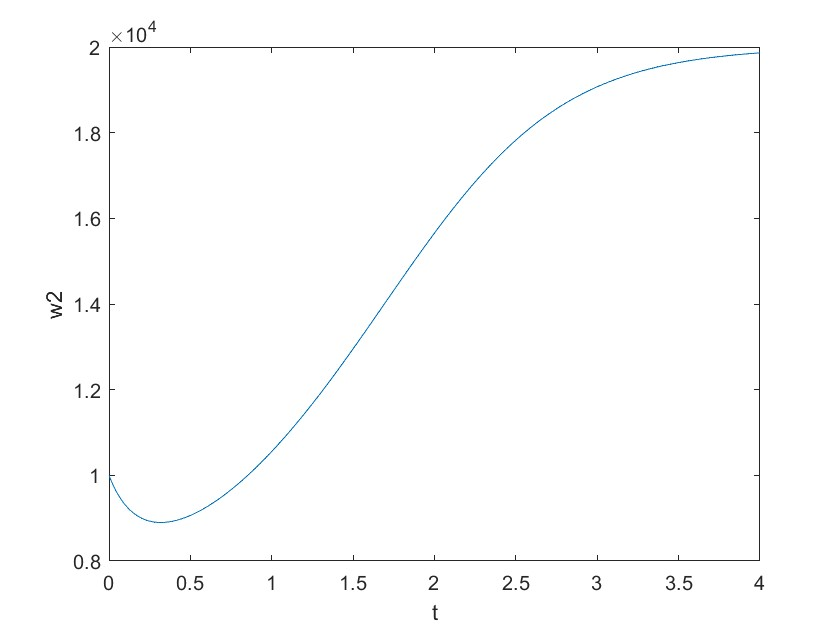
\includegraphics[width=\textwidth]{assignment_5_4_2_fig.jpg}
            \centering
            \caption{w2 graph}
        \end{subfigure}
        \caption{Plotting of w1 and w2 of RK4 method}
        \label{fig:RK4_Method_w1_And_w2_Graph}
    \end{figure} By observing the last 30 w1 and w2 values and the graph, we can see that the solution approach to constant, i.e., \begin{align}
        \begin{pmatrix} 
            x_1 \\
            x_2
        \end{pmatrix}
        \rightarrow
        \begin{pmatrix} 
            0 \\
            20000
        \end{pmatrix}
        \text{ as } t \rightarrow \infty.
    \end{align}
\end{enumerate}


\end{document}